% Created 2022-09-08 Thu 16:20
% Intended LaTeX compiler: pdflatex
\documentclass[11pt,a4paper]{article}
\usepackage{subfiles}
\usepackage{algorithm}
\usepackage{minted}
\usepackage{xcolor}
\usepackage[utf8]{inputenc}
\usepackage{gentium}
\usepackage{graphicx}
\usepackage{grffile}
\usepackage{longtable}
\usepackage{wrapfig}
\usepackage{rotating}
\usepackage[normalem]{ulem}
\usepackage{amsmath}
\usepackage{textcomp}
\usepackage{amssymb}
\usepackage{capt-of}
\usepackage{hyperref}
\usepackage[greek, english]{babel}
\usepackage{multicol}
\usepackage[framemethod=tikz]{mdframed}
\usepackage[compact]{titlesec}
\usepackage{float}
\titlespacing{ ection}{0pt}{*0}{*0}
\titlespacing{ ubsection}{0pt}{*0}{*0}
\titlespacing{ ubsubsection}{0pt}{*0}{*0}
\usepackage{geometry} % Required for adjusting page dimensions and margins
\geometry{
	paper=a4paper, % Paper size, change to letterpaper for US letter size
	top=2.5cm, % Top margin
	bottom=3cm, % Bottom margin
	left=2.5cm, % Left margin
	right=2.5cm, % Right margin
	headheight=14pt, % Header height
	footskip=1.5cm, % Space from the bottom margin to the baseline of the footer
	headsep=1.2cm, % Space from the top margin to the baseline of the header
	%showframe, % Uncomment to show how the type block is set on the page
}
\usepackage[utf8]{inputenc}
\usepackage[T1]{fontenc}
\usepackage{graphicx}
\usepackage{longtable}
\usepackage{wrapfig}
\usepackage{rotating}
\usepackage[normalem]{ulem}
\usepackage{amsmath}
\usepackage{amssymb}
\usepackage{capt-of}
\usepackage{hyperref}
\setcounter{secnumdepth}{3}
\author{Kostas Papadimos}
\date{}
\title{A Brief report of what I did the past week}
\hypersetup{
 pdfauthor={Kostas Papadimos},
 pdftitle={A Brief report of what I did the past week},
 pdfkeywords={},
 pdfsubject={},
 pdfcreator={Emacs 28.1 (Org mode 9.5.2)}, 
 pdflang={English}}
\begin{document}

\maketitle
\tableofcontents

\section{The problem}
\label{sec:org73da5ce}
There are two data sets(groups). Each data set consist of some  sets of 4 numbers. The sum of the numbers in each set of a group is the same.
The goal is to train a boosted decision tree such that it will be able to separate the numbers of each group.  
\section{Method}
\label{sec:orga5dafd6}
For simplicity, I was working with integer numbers. Moreover I created the the testing and training data sets in 3 different ways.
\begin{itemize}
\item I selected the number that every set of a given group will add up to
\item The sum of every set in a given group was selected randomly
\item The sum of every set in a given group was not the same. The numbers of each set summed to a number coming from a normal distribution
\end{itemize}
\subsection{Creating the data set}
\label{sec:org6702f83}
\subsubsection{Fixed sum}
\label{sec:orgef63043}
Having the number that each set of each group will add up to, I picked 3 random numbers in the range [-100, 100] and subtracted their sum from the fixed number. This way I created two groups of 10000 sets each.
\begin{verbatim}
def rand_data(s, n):
  '''
  returns n numbers, n1, n2, ... such that n1+n2+...=s
  '''
  import random as rand
  nums = [rand.randint(-100, 100) for i in range(n-1)]
  nums.append(s - sum(nums))
  return nums
#
s1, s2 = (2, 9) # randomly picked sum
n = 4 # numbers in each set
n_sets = 10000 # number of sets in each group
#
group_a = [rand_data(s, n) for i in range(n_sets)]
group_b = [rand_data(s, n) for i in range(n_sets)]
\end{verbatim}
In the histogram bellow, it is verified that the stets in each group add up to the same number.
\begin{figure}[htbp]
\centering
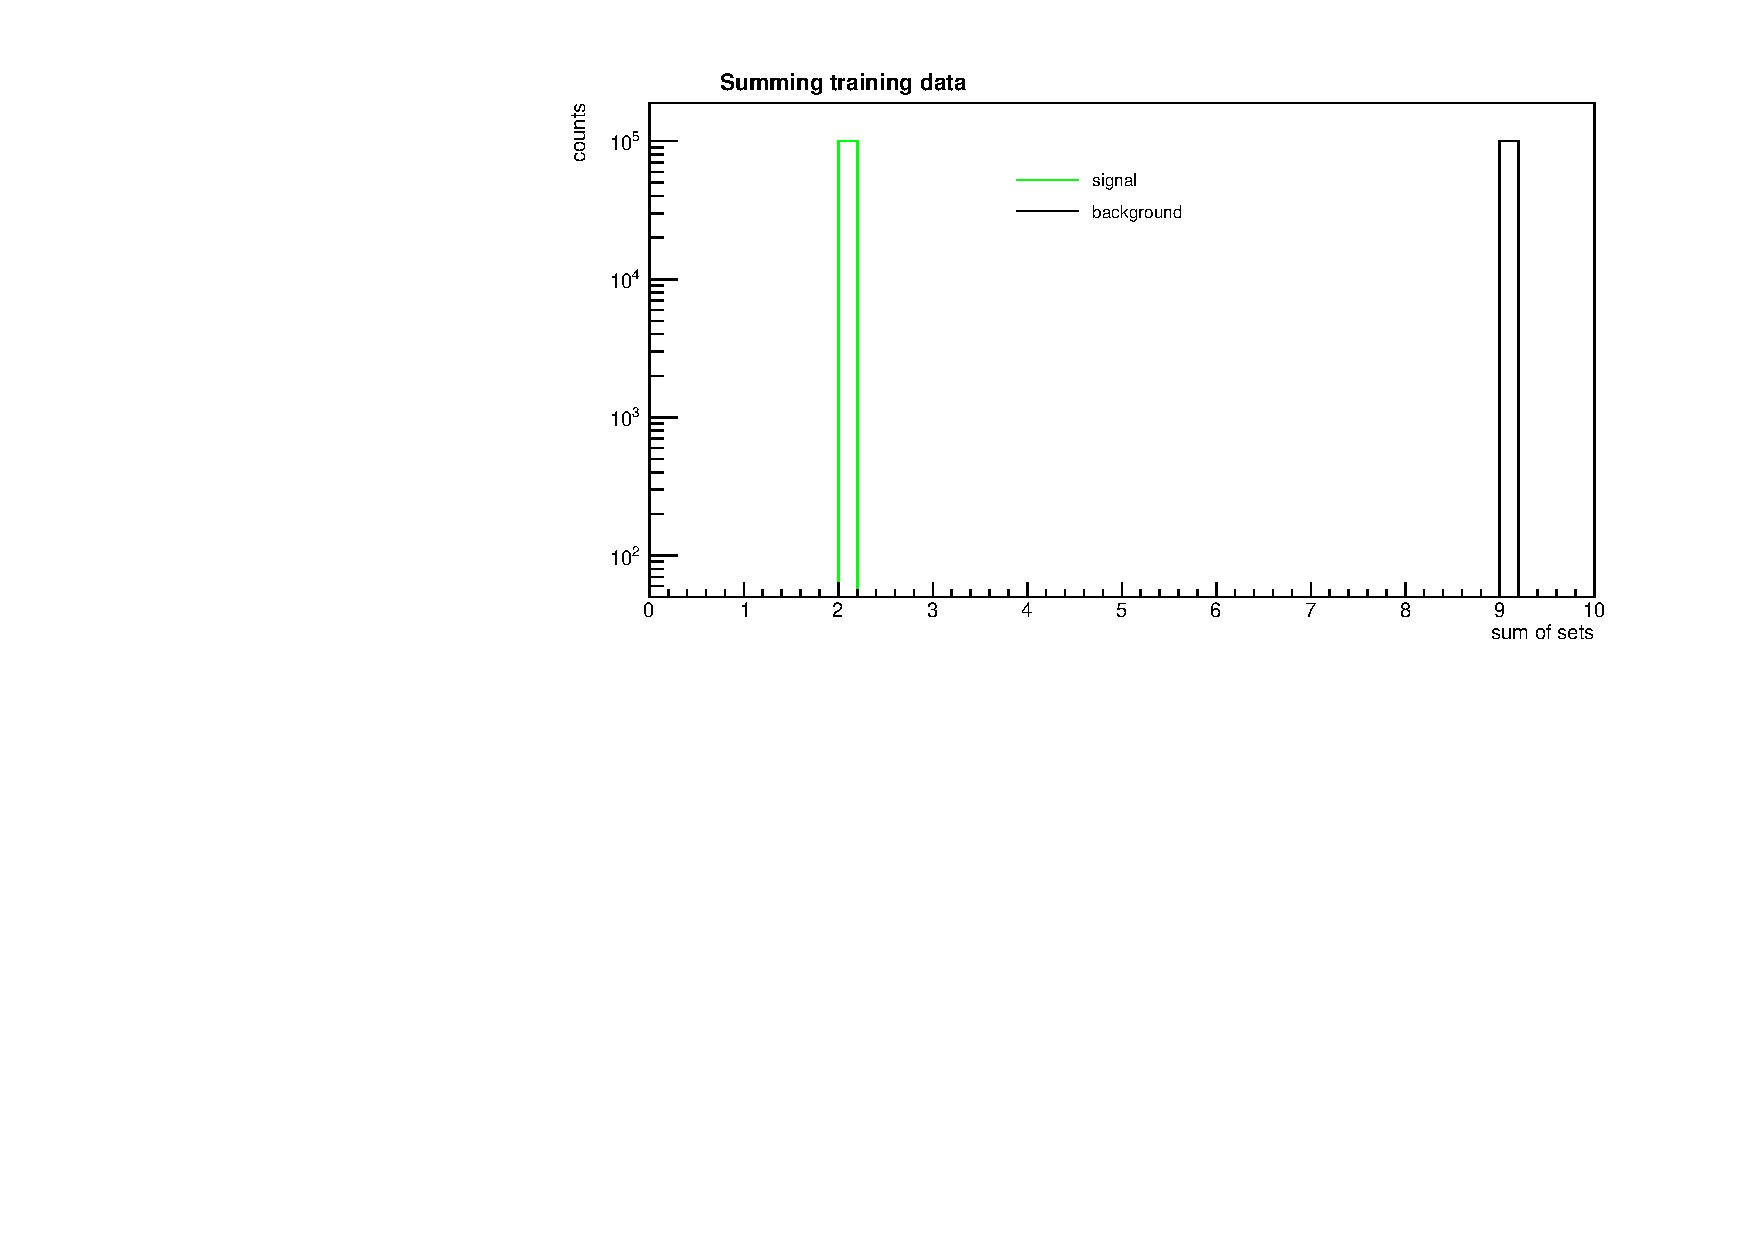
\includegraphics[width=.9\linewidth]{/home/kpapad/UG_thesis/tutorial_scripts/MachineLearning/Plots/trainingDatSum_twoNums.pdf}
\caption{\label{fig:org09df792}sum of each group. Using fixed sums}
\end{figure}

Obviously the sums of each group are s = 2 and s = 9.
\subsubsection{Random sum}
\label{sec:orgaa7bc0c}
The number that each set of each group will add up to, is not fixed by me, but its randomly selected in the range[0, 10], using a random number generator(python). The way of creating the numbers of each set is the same as before:
\begin{verbatim}
import random
s1, s2 = [random.randint(0, 10) for i in range(num_groups)] # randomly generated sum
n = 4 # numbers in each set
n_sets = 10000 # number of sets in each group
#
group_a = [rand_data(s, n) for i in range(n_sets)]
group_b = [rand_data(s, n) for i in range(n_sets)]
\end{verbatim}
In the histogram bellow, it is verified that the sets in each group add up to the same number.
\begin{figure}[htbp]
\centering
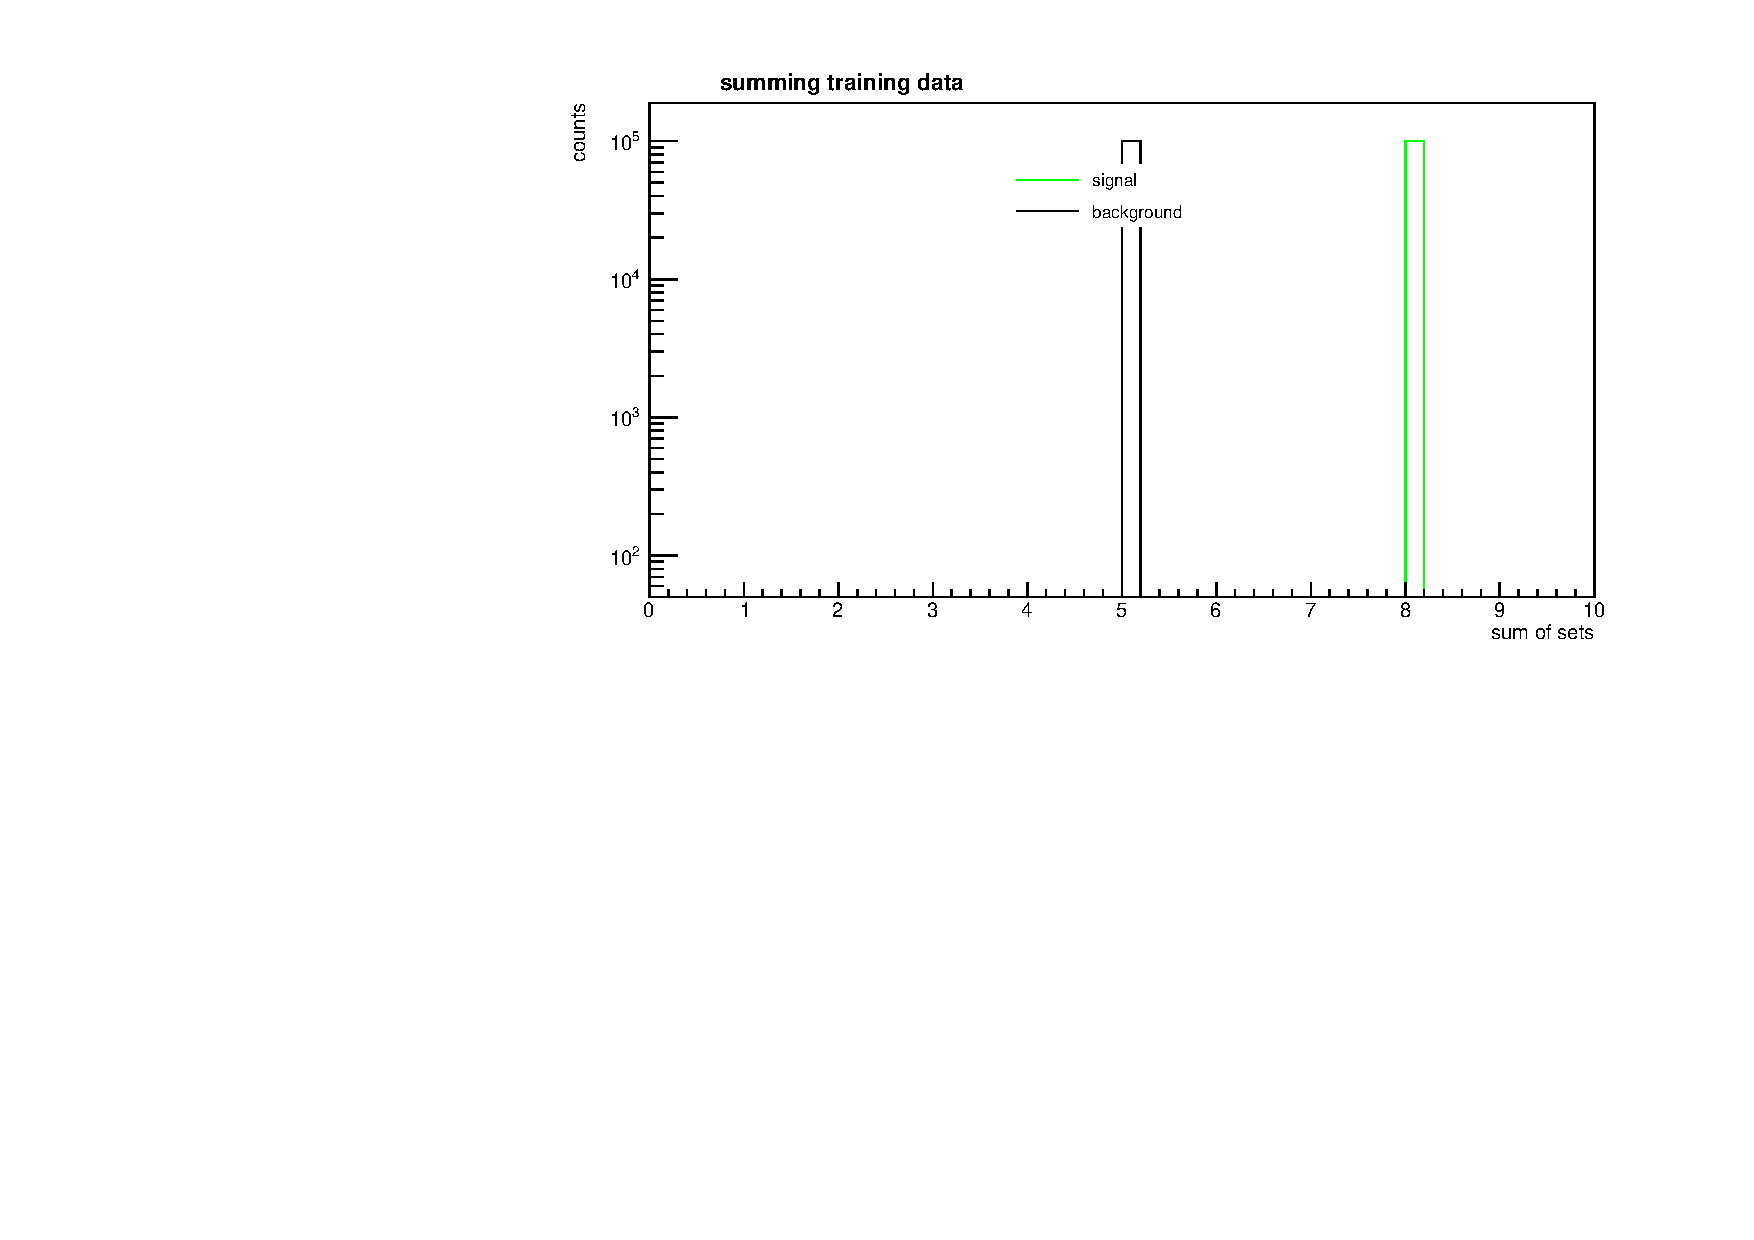
\includegraphics[width=.9\linewidth]{/home/kpapad/UG_thesis/tutorial_scripts/MachineLearning/Plots/rand.pdf}
\caption{\label{fig:org62d0142}sum of each group. Using random sums}
\end{figure}
Obviously the sums of each group are s = 5 and s = 8.
\newpage
\subsubsection{Normally distributed sum}
\label{sec:orgbf2f2a5}
The sets of a given group do not add up to the same number. Instead, the number that each set adds up to, follows the Gaussian distribution with fixed means and sigmas for each group:
\begin{verbatim}
mu_a, mu_b = (2, 9) # fixed means
sigma = 0.1 # for simplicity the sigma is kept the same
n_sets = 10000 # number of sets in each group
#
group_a = [rand_data(rand.gauss(mu_a, sigma), n) for i in range(n_sets)]
group_b = [rand_data(rand.gauss(mu_a, sigma), n) for i in range(n_sets)]
\end{verbatim}
In the histogram bellow, it is verified that the sets of a given group add up to a number thats normally distributed.
\begin{figure}[htbp]
\centering
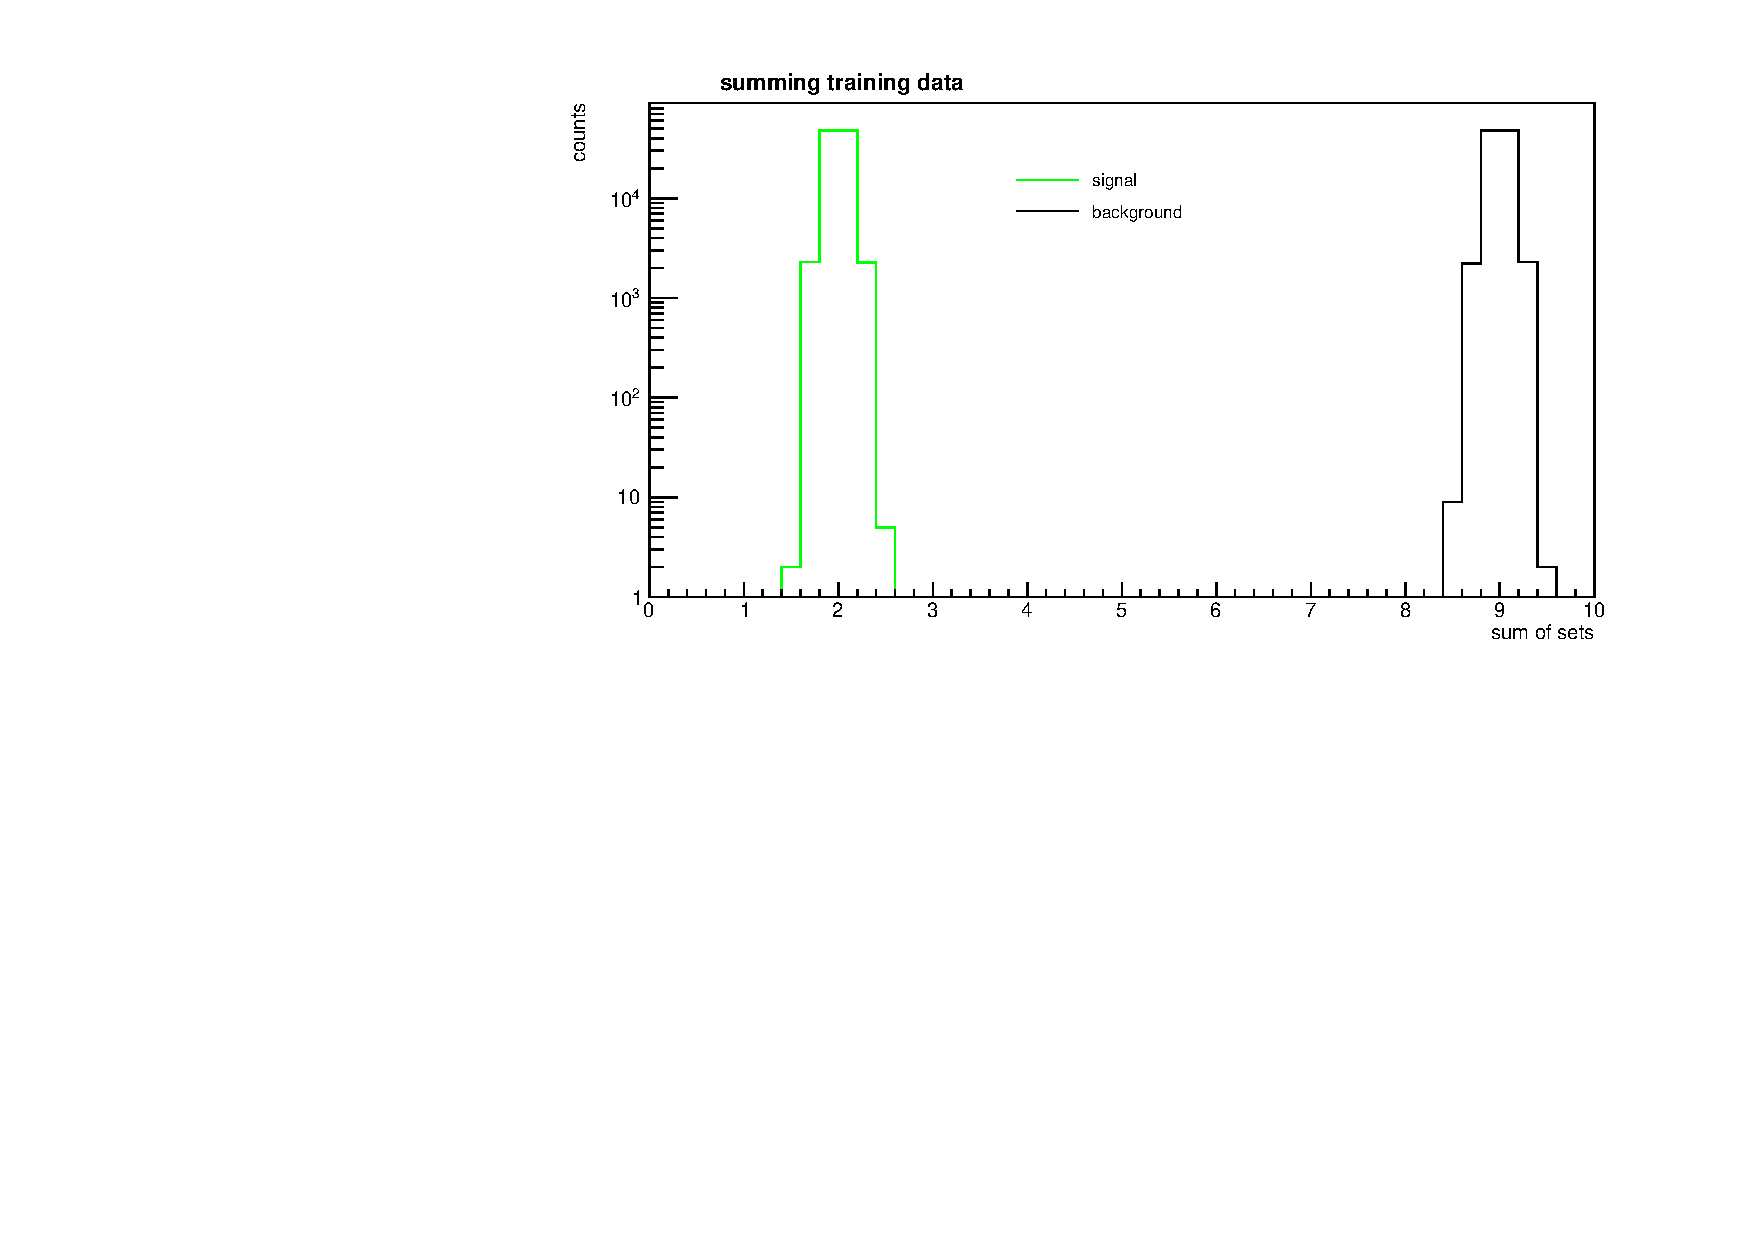
\includegraphics[width=.9\linewidth]{/home/kpapad/UG_thesis/tutorial_scripts/MachineLearning/Plots/dist.pdf}
\caption{\label{fig:org8df7416}sum of each group. Using normally distributed sums}
\end{figure}
The means of each distribution are \(\mu\) = 2 and \(\mu\) = 9 
\subsection{Testing and Training}
\label{sec:orgb7e5a42}
Both training and testing was done exactly as shown in the example at \url{https://root.cern.ch/doc/master/tmva101\_\_Training\_8py.html}.
\section{Results}
\label{sec:orge7ae33d}
The ROC curves as well as the AUC scores of each model are shown in the plot bellow:
\begin{figure}[htbp]
\centering
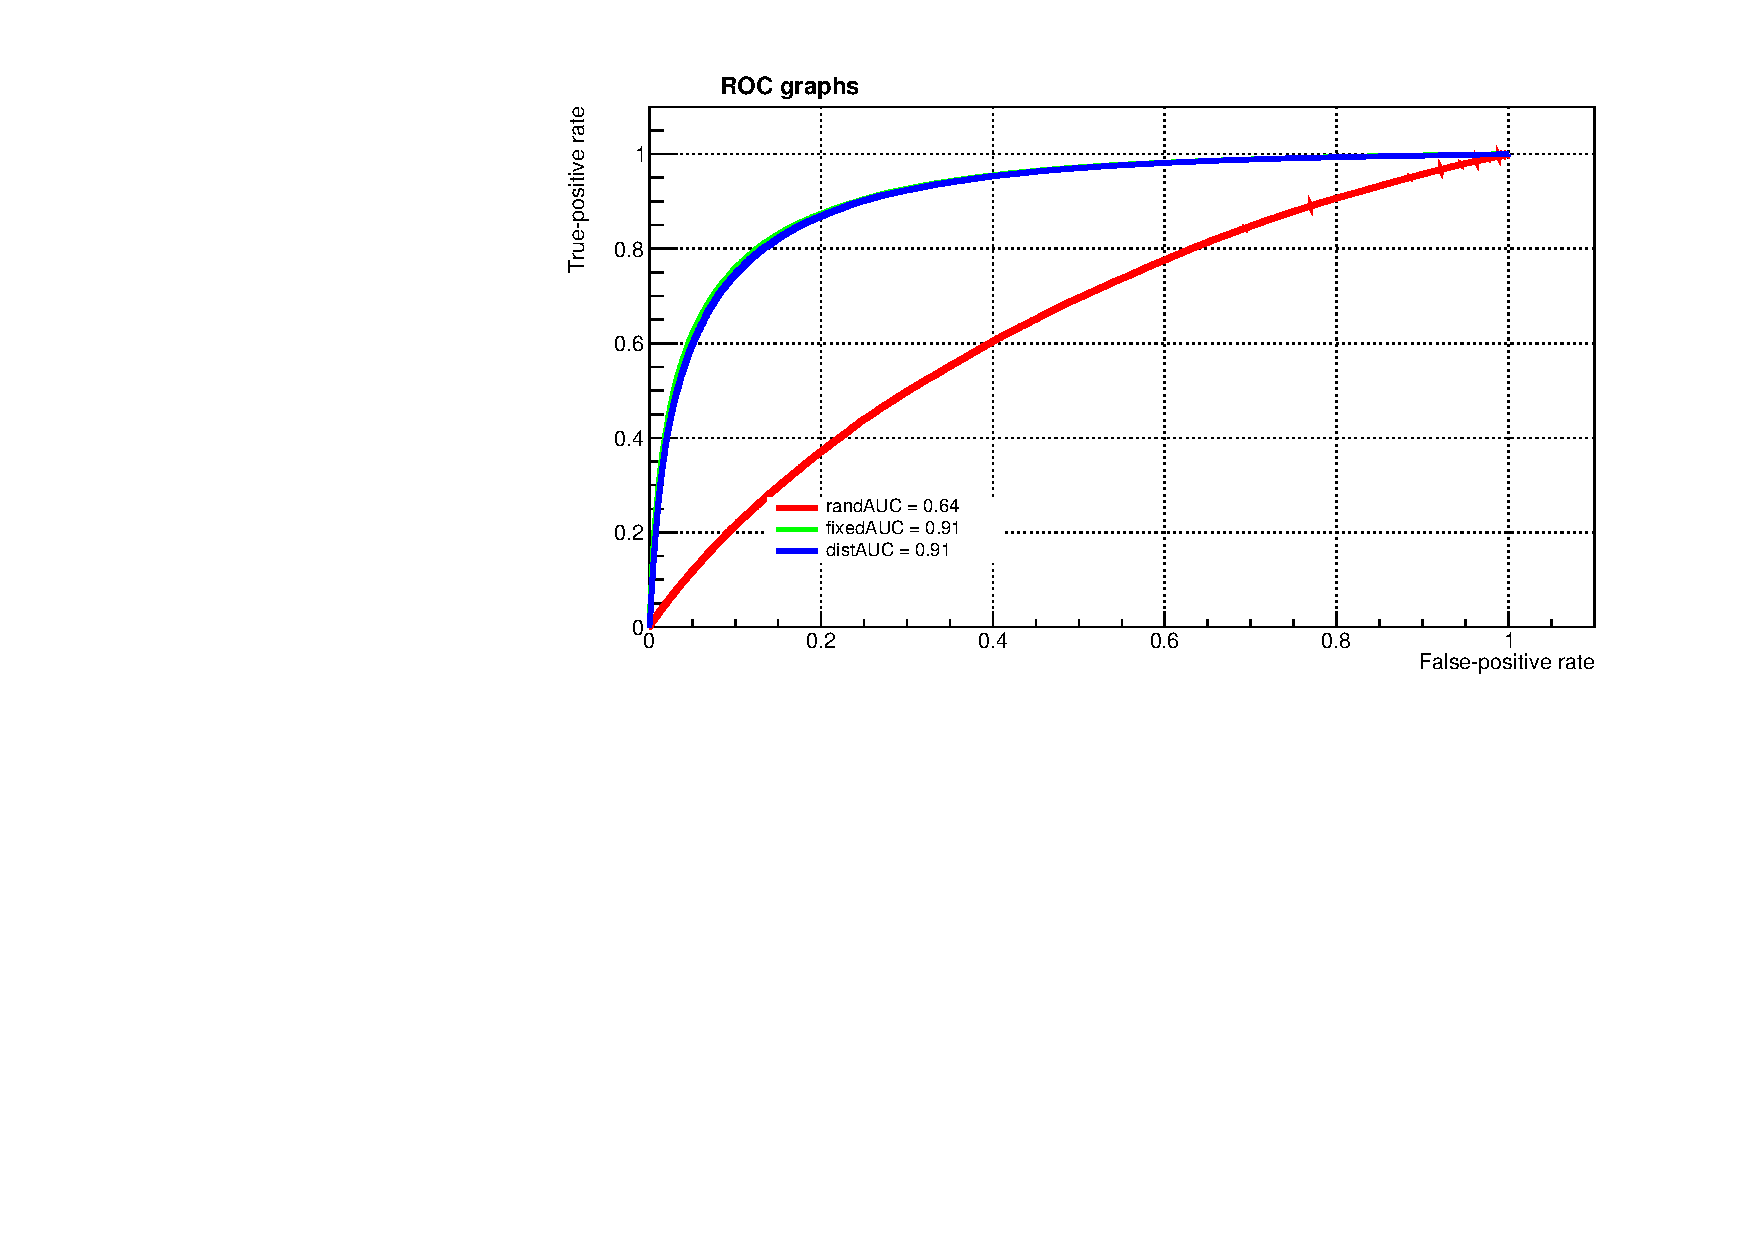
\includegraphics[width=.9\linewidth]{/home/kpapad/UG_thesis/tutorial_scripts/MachineLearning/unnamed.pdf}
\caption{\label{fig:orgb648629}Efficiency of each model based on the way that the data was generated}
\end{figure}
\end{document}